\chapter{Limits}

\section{Functions}{}{}

\fbox{This should be one of the last sections filled-in.}


\section{The Basic Ideas of Limits}{}{}


\begin{marginfigure}
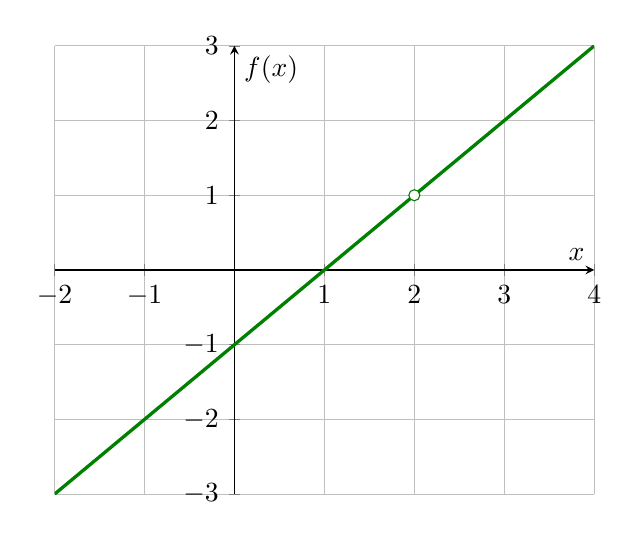
\begin{tikzpicture}
	\begin{axis}[
            domain=-2:4, xmax=4,
            axis lines =middle, xlabel=$x$, ylabel=$f(x)$,
            grid=both,
            xtick={-2,...,4},
            ytick={-3,...,3},
          ]
	  \addplot [very thick, green!50!black, smooth] {x-1};
          \addplot[color=green!50!black,fill=white,only marks,mark=*] coordinates{(2,1)}; 
        \end{axis}
\end{tikzpicture}
\caption{A plot of $f(x)=\protect\frac{x^2 - 3x + 2}{x-2}$.}
\label{plot:(x^2 - 3x + 2)/(x-2)}
\end{marginfigure}

\begin{margintable}
\[
\begin{array}{c|c}
 x & f(x) \\ \hline
 1.7 &  0.7 \\
 1.9 &  0.9 \\
 1.99 &  0.99 \\
 1.999 &  0.999 \\
  2 &  \text{undefined}
\end{array}\qquad
\begin{array}{c|c}
 x & f(x) \\ \hline
  2 & \text{undefined}\\
 2.001&  1.001\\
 2.01&  1.01\\
 2.1 &  1.1 \\
 2.3 &  1.3 \\
\end{array}
\]
\caption{Values of $f(x)=\protect\frac{x^2 - 3x + 2}{x-2}$.}
\label{table:(x^2 - 3x + 2)/(x-2)}
\end{margintable}
Consider the function:
\[
f(x) = \frac{x^2 - 3x + 2}{x-2}
\]
While $f(x)$ is undefined at $x=2$, we can still plot $f(x)$ at other
values, see Figure~\ref{plot:(x^2 - 3x + 2)/(x-2)}. Examining
Table~\ref{table:(x^2 - 3x + 2)/(x-2)}, we see that as $x$ approaces
$2$, $f(x)$ approaches $1$. We write this: As $x \to 2$, $f(x) \to 1$.
This leads us to the definition of a \textit{limit}.



\begin{definition}\label{def:limit} 
The \textbf{limit} of $f(x)$ as $x$ goes to $a$ is $L$,
\[
\lim_{x\to a}f(x)=L,
\] 
if for every $\epsilon>0$ there is a $\delta > 0$ so that whenever 
\[
a- \delta < x < a+ \delta, \qquad\text{we have} \qquad L-\epsilon< f(x)<L+\epsilon.
\] 
If no such value of $L$ can be
found, then we say that $f(x)$ \textbf{does not exist} at $x=a$.
\end{definition}

In Figure~\ref{figure:epsilon-delta}, we see a geometric
interperatation of this defintion.


\begin{figure}
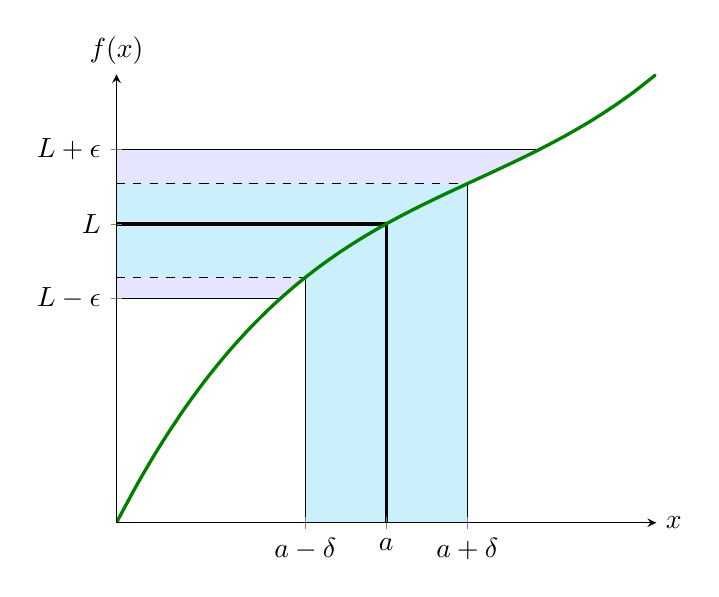
\begin{tikzpicture}
	\begin{axis}[
            domain=0:2, xmax=2,
            axis lines =left, xlabel=$x$, ylabel=$f(x)$,
            every axis y label/.style={at=(current axis.above origin),anchor=south},
            every axis x label/.style={at=(current axis.right of origin),anchor=west},
            xtick={0.7,1,1.3}, ytick={3,4,5},
            xticklabels={$a-\delta$,$a$,$a+\delta$}, yticklabels={$L-\epsilon$,$L$,$L+\epsilon$},
            axis on top,
            area style,
          ]          
          \addplot [fill=blue!10, smooth, domain=(0:1.570)] {5} \closedcycle;
          \addplot [black, smooth, domain=(0:1.570)] {5};
          \addplot [fill=cyan!20, dashed, smooth, domain=(0:1.3)] {4.537} \closedcycle;
          \addplot [fill=blue!10, dashed, domain=(0:.7)] {3.283} \closedcycle;       
          \addplot [black, dashed, smooth, domain=(0:1.570)] {4.537};
          \addplot [black, dashed, smooth, domain=(0:1.570)] {3.283};
          \addplot [black, very thick, smooth, domain=(0:1)] {4};
          \addplot [fill=white, smooth, domain=(0:0.607)] {3} \closedcycle;
          \addplot [black, smooth, domain=(0:0.607)] {3};
	  \addplot [fill=white, smooth,domain=(0:3)] {x*(x-2)^2+3*x} \closedcycle;
          \addplot [fill=cyan!20, draw=none, domain=.7:1.3] {x*(x-2)^2+3*x} \closedcycle;
          \addplot [black, very thick] plot coordinates {(1,0) (1,4)};
          \addplot [black] plot coordinates {(.7,0) (.7,3.283)};
          \addplot [black] plot coordinates {(1.3,0) (1.3,4.537)};
	  \addplot [very thick,green!50!black, smooth] {x*(x-2)^2+3*x};
        \end{axis}
\end{tikzpicture}
\caption{A geometric interpertation of the $\epsilon$-$\delta$
  criterion for limits.  Here we see that for every $x$ such that $a
  -\delta < x < a+\delta$, we are sure to have $L - \epsilon< f(x) <
  L+\epsilon$.}
\label{figure:epsilon-delta}
\end{figure}


\fbox{Examples with numbers}


\begin{example} Show that $\ds \lim_{x\to 2} x^2=4$.
 
We want to show that for any given $\epsilon>0$, we can find a
$\delta>0$ such that $\ds |x^2-4|<\epsilon$ whenever $0<|x-2|<\delta$.

Write $\ds |x^2-4|=|(x+2)(x-2)|$. Now when $|x-2|$ is small, part of
$|(x+2)(x-2)|$ is small, namely $(x-2)$. What about $(x+2)$? If $x$ is
close to 2, $(x+2)$ certainly can't be too big, but we need to somehow
be precise about it. Let's recall the ``game'' version of what is
going on here. You get to pick an $\epsilon$ and I have to pick a
$\delta$ that makes things work out. Presumably it is the really tiny
values of $\epsilon$ I need to worry about, but I have to be prepared
for anything, even an apparently ``bad'' move like $\epsilon=1000$.  I
expect that $\epsilon$ is going to be small, and that the
corresponding $\delta$ will be small, certainly less than 1.  If
$\delta\le 1$ then $|x+2|<5$ when $|x-2|<\delta$ (because if $x$ is
within 1 of 2, then $x$ is between 1 and 3 and $x+2$ is between 3 and
5). So then I'd be trying to show that
$|(x+2)(x-2)|<5|x-2|<\epsilon$. So now how can I pick $\delta$ so that
$|x-2|<\delta$ implies $5|x-2|<\epsilon$? This is easy: use
$\delta=\epsilon/5$, so $5|x-2|<5(\epsilon/5) = \epsilon$. But what if
the $\epsilon$ you choose is not small? If you choose $\epsilon=1000$,
should I pick $\delta=200$? No, to keep things ``sane'' I will never
pick a $\delta$ bigger than 1. Here's the final ``game strategy:''
When you pick a value for $\epsilon$ I will pick $\delta=\epsilon/5$
or $\delta=1$, whichever is smaller. Now when $|x-2|<\delta$, I know
both that $|x+2|<5$ and that $|x-2|<\epsilon/5$. Thus
$|(x+2)(x-2)|<5(\epsilon/5) = \epsilon$.

This has been a long discussion, but most of it was explanation and
scratch work. If this were written down as a proof, it would be quite
short, like this:

Proof that $\ds \lim_{x\to 2}x^2=4$. Given any $\epsilon$, pick
$\delta=\epsilon/5$ or $\delta=1$, whichever is smaller. Then when
$|x-2|<\delta$, $|x+2|<5$ and
$|x-2|<\epsilon/5$. Hence $\ds |x^2-4|=|(x+2)(x-2)|<5(\epsilon/5) =
\epsilon$. 
\end{example}







\begin{exercises}

Compute the limits. If a limit does not exist, explain why.

\twocol

\begin{exercise} $\ds \lim_{x\to 3}{x^2+x-12\over x-3}$
\begin{answer} 7
\end{answer}\end{exercise}

\begin{exercise} $\ds \lim_{x\to 1}{x^2+x-12\over x-3}$
\begin{answer} 5
\end{answer}\end{exercise}

\begin{exercise} $\ds \lim_{x\to -4}{x^2+x-12\over x-3}$
\begin{answer} 0
\end{answer}\end{exercise}

\begin{exercise} $\ds \lim_{x\to 2} {x^2+x-12\over x-2}$
\begin{answer} undefined
\end{answer}\end{exercise}

\begin{exercise} $\ds \lim_{x\to 1} {\sqrt{x+8}-3\over x-1}$
\begin{answer} $1/6$
\end{answer}\end{exercise}

\begin{exercise} $\ds \lim_{x\to 0^+} \sqrt{{1\over x}+2} - \sqrt{1\over x}$.
\begin{answer} 0
\end{answer}\end{exercise}

\begin{exercise} $\ds\lim _{x\to 2} 3$
\begin{answer} 3
\end{answer}\end{exercise}

\begin{exercise} $\ds\lim _{x\to 4 } 3x^3 - 5x $
\begin{answer} 172
\end{answer}\end{exercise}

\begin{exercise} $\ds \lim _{x\to 0 } {4x - 5x^2\over x-1}$
\begin{answer} 0
\end{answer}\end{exercise}

\begin{exercise} $\ds\lim _{x\to 1 } {x^2 -1 \over x-1 }$
\begin{answer} 2
\end{answer}\end{exercise}

\begin{exercise} $\ds\lim _{x\to 0^ + } {\sqrt{2-x^2 }\over x}$
\begin{answer} does not exist
\end{answer}\end{exercise}

\begin{exercise} $\ds\lim _{x\to 0^ + } {\sqrt{2-x^2}\over x+1}$
\begin{answer} $\ds \sqrt2$
\end{answer}\end{exercise}

\begin{exercise} $\ds\lim _{x\to a } {x^3 -a^3\over x-a}$
\begin{answer} $\ds 3a^2$
\end{answer}\end{exercise}

\begin{exercise} $\ds\lim _{x\to 2 } (x^2 +4)^3$
\begin{answer} 512
\end{answer}\end{exercise}

\begin{exercise} $\ds\lim _{x\to 1 } \begin{cases}
x-5 & x\neq 1, \\
7 & x=1. \end{cases}$
\begin{answer} $-4$
\end{answer}\end{exercise}

\endtwocol

\msk
\begin{exercise} $\ds\lim _{x\to 0 } x\sin \left( {1\over x}\right)$
(Hint: Use the fact that $|\sin a |< 1 $ for any real number $a$. You
should probably use the definition of a limit here.)
\begin{answer} $0$
\end{answer}\end{exercise}

\begin{exercise} Give an $\epsilon$--$\delta$ proof, similar to
example~\xrefn{exam:epsilon-delta proof},
of the fact that 
$\ds \lim_{x\to 4} (2x-5) = 3$. 
\end{exercise}

\begin{exercise} Evaluate the expressions by reference to this graph:\hfill\break
BADBAD

% BADBAD
%\hbox{\epsfxsize8cm\epsfbox{limit-exercise-graph.eps}}\hfill\break

% \halign{&\indent#\hfill \\
%  (a) $\ds \lim_{x\to 4} f(x)$ & 
%  (b) $\ds \lim_{x\to -3} f(x)$ & 
%  (c) $\ds \lim_{x\to 0} f(x)$  \\
%  (d) $\ds \lim_{x\to 0^-} f(x)$ & 
%  (e) $\ds \lim_{x\to 0^+} f(x)$ & 
%  (f) $\ds f(-2)$  \\
%  (g) $\ds \lim_{x\to 2^-} f(x)$ & 
%  (h) $\ds \lim_{x\to -2^-} f(x)$ & 
%  (i) $\ds \lim_{x\to 0} f(x+1)$  \\
%  (j) $\ds f(0)$ & 
%  (k) $\ds \lim_{x\to 1^-} f(x-4)$ & 
%  (l) $\ds \lim_{x\to 0^+} f(x-2)$  \\}
% \begin{answer} (a) $8$, (b) $6$, (c) dne, (d) $-2$, (e) $-1$, (f) $8$,
%  (g) $7$, (h) $6$, (i) $3$, (j) $-3/2$, (k) $6$, (l) $2$
% \end{answer}
\end{exercise}

\begin{exercise} Use a calculator to estimate $\ds\lim_{x\to 0}
{\sin x\over x}$.
\end{exercise}

\begin{exercise} Use a calculator to estimate $\ds\lim_{x\to 0}
{\tan(3x)\over\tan(5x)}$.
\end{exercise}
\end{exercises}






\section{Limit Laws}

\begin{theorem} 
Suppose $\ds \lim_{x\to a} f(x)=L$ and $\ds \lim_{x\to a}g(x)=M$. Then
$\lim_{x\to a} f(x)g(x) = LM$.
\end{theorem}

\begin{proof} 
Given any $\epsilon$ we need to find a $\delta$ so that
$0<|x-a|<\delta$ implies $|f(x)g(x)-LM|<\epsilon$. What do we have to
work with? We know that we can make $f(x)$ close to $L$ and $g(x)$
close to $M$, and we have to somehow connect these facts to make
$f(x)g(x)$ close to $LM$.

We use, as is so often the case, a little algebraic
trick: 
\begin{align*}
|f(x)g(x)-LM| &= |f(x)g(x)\boldsymbol{-f(x)M+f(x)M}-LM| \\
&=|f(x)(g(x)-M)+(f(x)-L)M| \\
&\le |f(x)(g(x)-M)|+|(f(x)-L)M| \\
&=|f(x)||g(x)-M|+|f(x)-L||M|.
\end{align*}

This is all straightforward except perhaps for the ``$\le$''. That is
an example of the {\dfont triangle inequality%
\index{triangle inequality}\pagerdef{page:triangle inequality}}, 
which says that if $a$ and $b$ are any real
numbers then $|a+b|\le |a|+|b|$. If you look at a few examples, using
positive and negative numbers in various combinations for $a$ and $b$,
you should quickly understand why this is true; we will not prove it
formally. 

Since $\ds \lim_{x\to a}f(x) =L$, there is a value $\ds \delta_1$ so that
$0<|x-a|<\delta_1$ implies $|f(x)-L|<|\epsilon/(2M)|$, 
This means that $0<|x-a|<\delta_1$ implies
$|f(x)-L||M|< \epsilon/2$. You can see where this is going: if we can
make $|f(x)||g(x)-M|<\epsilon/2$ also, then we'll be done.

We can make $|g(x)-M|$ smaller than any fixed number by making $x$
close enough to $a$; unfortunately, $\epsilon/(2f(x))$ is not a fixed
number, since $x$ is a variable. Here we need another little trick,
just like the one we used in analyzing $x^2$. We can find a $\delta_2$
so that $|x-a|<\delta_2$ implies that $|f(x)-L|<1$, meaning that $L-1
< f(x) < L+1$. This means that $|f(x)|<N$, where $N$ is either $|L-1|$
or $|L+1|$, depending on whether $L$ is negative or positive. The
important point is that $N$ doesn't depend on $x$. Finally, we know that
there is a $\delta_3$ so that $0<|x-a|<\delta_3$ implies
$|g(x)-M|<\epsilon/(2N)$. Now we're ready to put everything
together. Let $\delta$ be the smallest of $\delta_1$, $\delta_2$, and
$\delta_3$. Then $|x-a|<\delta$ implies that
$|f(x)-L|<|\epsilon/(2M)|$, $|f(x)|<N$, and
$|g(x)-M|<\epsilon/(2N)$. Then 
\begin{align*}
|f(x)g(x)-LM|&\le|f(x)||g(x)-M|+|f(x)-L||M| \\
&<N{\epsilon\over 2N}+\left|{\epsilon\over 2M}\right||M| \\
&={\epsilon\over 2}+{\epsilon\over 2}=\epsilon.
\end{align*}
This is just what we needed, so by the official definition,
$\ds \lim_{x\to a}f(x)g(x)=LM$.
\end{proof}

A handful of such theorems give us the tools to compute many limits
without explicitly working with the definition of limit.

\begin{theorem}[Limit Laws] Suppose that $\ds \lim_{x\to a}f(x)=L$ and $\ds \lim_{x\to a}g(x)=M$ and
$k$ is some constant. Then
\begin{itemize}
\item $\ds\lim_{x\to a} kf(x) = k\lim_{x\to a}f(x)=kL$ 
\item $\ds\lim_{x\to a} (f(x)+g(x)) = \lim_{x\to a}f(x)+\lim_{x\to a}g(x)=L+M$  
\item $\ds\lim_{x\to a} (f(x)g(x)) = \lim_{x\to a}f(x)\cdot\lim_{x\to a}g(x)=LM$ 
\item $\ds\lim_{x\to a} \frac{f(x)}{g(x)} = \frac{\ds\lim_{x\to a}f(x)}{\ds\lim_{x\to
    a}g(x)}=\frac{L}{M},\text{ if $M$ is not 0}$
\end{itemize}
\label{thm:limit laws}
\end{theorem}

Roughly speaking, these rules say that to compute the limit of an
algebraic expression, it is enough to compute the limits of the
``innermost bits'' and then combine these limits. This often means
that it is possible to simply plug in a value for the variable, since
$\ds \lim_{x\to a} x =a$.
